% !TEX root = ../main.tex
\section{Motivation}
\label{sec:motivation}

We examine where a reasoning agent spends its time once speculative tool dispatch is in place.
The analysis uses the runs of speculative tool dispatch from \cref{sec:experiments} under deterministic serving: Qwen3-32B on the airline and retail domains of \taubench, with \MotTasks{} tasks, \MotTurns{} turns, and a \ToolLowFloor\,s floor on tool latency.
\Cref{app:results} repeats it for standard serving, where turns are shorter and the picture is the same.

\subsection{The Slack Can Hold the Next Turn}
\label{sec:motivation:slack}

Speculative tool dispatch settles the tool call early.
In \MotAnchorTurns{} of the \MotToolTurns{} tool-calling turns (\MotAnchorPct\%), a call is dispatched during reasoning and equals the call that the model finally emits.
In these turns the observation is ready after a median of \MotReadyPosPct\% of the turn's generation time.
The model then keeps reasoning.
We call the time from the moment the observation is ready to the end of the turn's generation the \emph{slack}.
Its median is \MotSlackMedian\,s, which is \MotSlackSharePct\% of the turn's generation time, and the slack of all these turns adds up to \MotSlackWallPct\% of the end-to-end time.
Tool execution, in contrast, amounts to only \MotToolGenPct\% of the generation time.
ETA reports the same pattern in a similar setting~\citep{anon2026eta}.
Reusing the probe's tokens as drafts when the model writes its call is bounded in the same way: the accepted draft tokens are \MotDraftTokenPct\% of all generated tokens.

We ask a further question about the slack: is it long enough to do the work of the next turn?
\Cref{fig:slack} compares each slack with the duration of the turn that follows.
The median next turn takes \MotNextMedian\,s, and the median ratio of slack to next-turn duration is \MotSlackOverNext.
In \MotNextFitsPct\% of the \MotPairs{} pairs the whole next turn would fit into the slack, and in \MotNextHalfPct\% at least half of it would.
On average, \MotNextCoveredPct\% of the next turn could run inside the slack.

\begin{figure}[t]
\centering
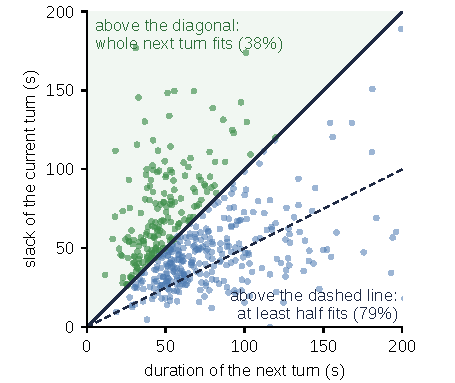
\includegraphics[width=\columnwidth]{figures/fig2_slack.pdf}
\caption{Slack of a turn against the duration of the turn that follows, for the \MotPairs{} pairs of consecutive turns in which the dispatched call was correct (Qwen3-32B, \taubench). \MotPlotOutside{} pairs beyond 200\,s are not shown.}
\label{fig:slack}
\end{figure}

\subsection{The Next Input Is Already Determined}
\label{sec:motivation:input}

Running the next turn early requires its input.
That input is the conversation so far plus what the current turn adds to it.
The turn's reasoning is not part of what is added.
The model developers recommend that the history keep only the final output of each turn, without its thinking content~\citep{qwen2025qwen3card,qwen2026qwen35card}, and agent harnesses follow this practice~\citep{bai2026spork,xu2026leap}.\footnote{The reference chat templates of both models re-insert reasoning that the caller supplies for assistant turns after the last user message. Our harness never supplies it, for any method.}
A tool-calling turn therefore adds only its visible output, which is normally the call alone, and the observation.
Both are available during the slack: the call has been predicted, and the observation has been obtained by executing it.

We test this on the same \MotAnchorTurns{} turns.
For each turn, we build the next input from the dispatched call and its observation alone and compare it with the input that the agent actually used.
The two are identical, token by token, in \MotInputSame{} cases (\MotInputSamePct\%).
In the other \MotInputDiff{}, the model's output contained more than the call: visible text before the call (\MotInputText{} cases) or a malformed closing tag that stayed in the history (\MotInputTag{} cases).

\subsection{Challenges}
\label{sec:motivation:challenges}

The two observations suggest starting the next turn inside the slack.
Doing so without changing the agent's behavior raises three challenges.

\paragraph{When to start, and from which input.}
The current turn has not finished when the next one should start, so its final call is unknown.
A correct call has been dispatched in \MotAnchorPct\% of the tool-calling turns, but not in the rest.
The next turn must start from an input that is available early and is likely to be the real one.

\paragraph{Side effects.}
A turn that starts early calls tools of its own before anyone knows whether it will be kept.
Some of these calls change state.
In the \method runs of \cref{sec:experiments}, \MotStateTotal{} early turns changed the database, for example through returns or flight changes, and discarded turns account for \MotStateDiscarded{} of them.
Such calls must not reach the real environment before the turn is confirmed.

\paragraph{When to keep the result.}
A matching call does not guarantee a matching input (\cref{sec:motivation:input}).
A turn that ran on a different input is not the turn the serial agent would have produced, and keeping it would change the trajectory.

\Cref{sec:method} addresses these challenges with \stratLaunch, \stratSandbox, and \stratCommit, respectively.
